\chapter{Lecture 10 - Brayton Cycle Review}
\label{ch:ch10}
\section{Objectives}
The objectives of this lecture are:
\begin{itemize}
\item Review the processes for a simple Brayton cycle
\item Carry out example analysis using:
\begin{itemize}
\item a constant specific heat approach; and
\item using EasyProp
\end{itemize}
\end{itemize}

\index{Brayton cycle}
\section{Brayton Cycle Review}
The Brayton cycle is a fundamental heat-engine thermodynamic cycle that is widely used to model gas turbine engines used for helicopters, tanks, and of course power plants. A schematic of a simple direct variant of the Brayton cycle for nuclear energy conversion is shown in Figure \ref{fig:simple_brayton}. Similar to a Rankine cycle the simplest version has the following processes:
\begin{marginfigure}
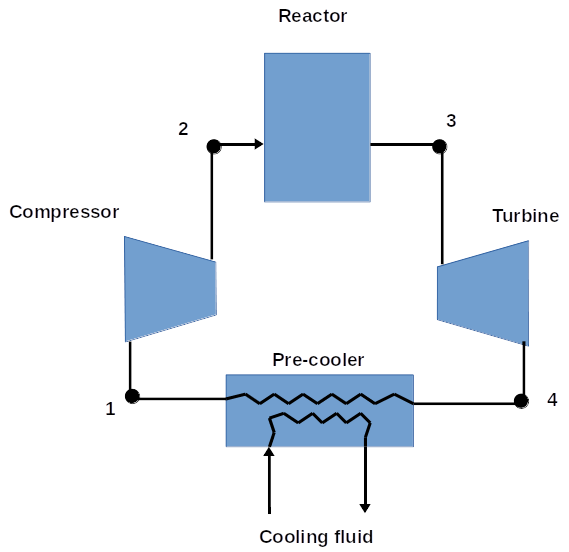
\includegraphics{simple_brayton.png}
\caption{A simple direct Brayton cycle for nuclear energy conversion.} 
\label{fig:simple_brayton}
\end{marginfigure}
\begin{enumerate}
\item isentropic compression ($ 1 \rightarrow 2$)
\item isobaric heat addition ($ 2 \rightarrow 3$)
\item isentropic expansion ($3 \rightarrow 4$)
\item isobaric heat rejection ($4 \rightarrow 1$)

\end{enumerate}
These are the same processes as a Rankine cycle; the difference is that the working fluid does not undergo a phase change during either heat addition or heat rejection; the working fluid is modeled as a compressible gas.  The temperature-entropy diagram for a non-ideal variation of the cycle is shown in Figure \ref{fig:simple_brayton_TS}.  For this, the compressor and turbine both are non-isentropic.
\begin{marginfigure}
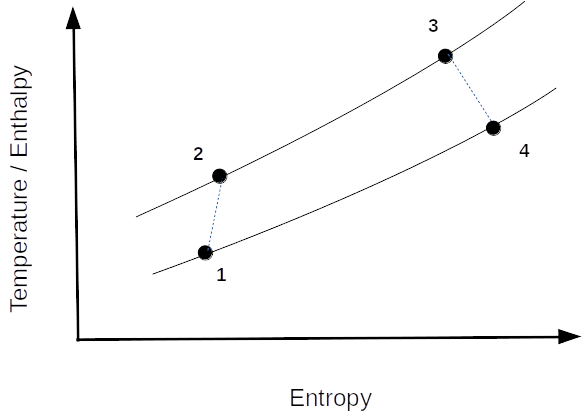
\includegraphics{simple_brayton_TS.png}
\caption{Temperature-Entropy diagram for a simple non-ideal Brayton cycle.}
\label{fig:simple_brayton_TS}
\end{marginfigure}

A more accurate representation of the cycle would also account for inevitable hydraulic losses as the working fluid flows through ducting and heat exchangers associated with the cycle.  For a Rankine cycle using water as the working fluid, these loss mechanisms are comparatively small but for Brayton cycle these losses are important and have a large impact on overall system thermodynamic performance.

\section{Analysis of Ideal Brayton Cycle - Constant Specific Heat}

If we assume the working fluid is an ideal gas in which the specific heat at constant pressure $(C_p)$ and constant volume $(C_v)$ are both assumed to be constant, an analytic solution method is feasible. We will model changes in enthalpy using the relationship given in Equation \ref{eq:IG_dh}.

\begin{equation}
\Delta h = C_p \Delta T
\label{eq:IG_dh}
\end{equation}

For isentropic processes a relationship exists between initial and final temperature of the working fluid, and the initial and final pressure of the working fluid. This relationship is given in Equation \ref{eq:IG_isentropic}.


\begin{equation}
\frac{T_f}{T_i} = \left(\frac{P_f}{P_i} \right)^{\frac{\gamma - 1}{\gamma}} = r_p^{\frac{P_f}{P_i}}
\label{eq:IG_isentropic}
\end{equation}


where $\gamma$ is the ratio of specific heats and $r_p$ is referred to as the ``pressure ratio.''\marginnote{\textbf{Note: }$\gamma = \sfrac{C_p}{C_v}$, and $r_p = \sfrac{P_f}{P_i}$}.  


\begin{example}
\textbf{Example:} Consider the a simple, ideal, closed, direct nuclear Brayton cycle.  Assuming the coolant is helium with $c_p=5.23 \text{ kJ/kg-}^{\circ}\text{K}$ and $\gamma=1.658$.  The maximum cycle temperature is 972 K and minimum temperature is 278 K.  The compressor pressure ratio is 4.0.  Find:
\begin{enumerate}
\item net specific work
\item thermal efficiency; and
\item back work ratio
\end{enumerate}
\end{example}

\begin{fullwidth}
\textbf{Solution:} 
Work of the isentropic compressor and turbine can be found by combining Equation \ref{eq:IG_dh} and Equation \ref{eq:IG_isentropic}.  

For the compressor we get:
$$w_c = h_1 - h_2 = C_p(T_1 - T_2) = C_p(T_1 - T_1 r_p^{\sfrac{\gamma - 1}{\gamma}}) = C_p T_1 (1 - r_p^{\sfrac{\gamma - 1}{\gamma}})$$
Applying the given numbers gives us:
$$w_c = (5.23 \text{kJ/kg-K})(273 \text{K})(1-4^{\sfrac{0.658}{1.658}}) = -1066.5 \text{kJ/kg}$$
For the turbine we get:
$$W_t = h_3 - h_4 = C_p(T_3 - T_4) = C_p(T_3 - T_3(\frac{1}{r_p})^{\frac{\gamma-1}{\gamma}}] = C_p T_3 [1 - (\frac{1}{r_p})^{\sfrac{\gamma-1}{\gamma}}]$$
which comes to:
$$w_t = (5.23 \text{kJ/kg-K})(972 \text{K})(1 - 0.25^{\frac{0.658}{1.658}}) = 2151.1 \text{kJ/kg}$$
net specific work is thus: $w_{\text{net}}=-1066.5 + 2151.1 = 1084.3 \text{kJ/kg}$.

\vspace{0.5cm}

We should calculate net specific heat added in order to compare with net work; for this we need values for the temperature at state points 2 and 4.  Using Equation \ref{eq:IG_isentropic} we get $T_2 = T_1 r_p^{\sfrac{\gamma-1}{\gamma}} = 278(4)^{\sfrac{0.658}{1.658}}=481.9$K and $T_4 = T_3 (\sfrac{1}{r_p})^{\sfrac{\gamma - 1}{\gamma}} = 972(0.25)^{\sfrac{0.658}{1.658}} = 560.7$K.  
Using these numbers with Equation \ref{eq:IG_dh} we get: $q_r = h_1 - h_4 = C_p(T_1 - T_4) = 5.23 \text{kJ/kg-K}(278 - 560.7) = -1478.5$kJ/kg and $q_s = h_3 - h_2 = C_p(T_3 - T_2) = 5.23 \text{kJ/kg-K}(972 - 481.9) = 2563.2$kJ/kg. 
Net specific heat added is, therefore: $q_{\text{net}} = q_s + q_r = 2563.1 - 1478.5 = 1084.7$kJ/kg which is very close to our calculated value for $w_{\text{net}}$.  

\vspace{0.5cm}
Thermal efficiency is given as $\eta_{th} = \sfrac{w_{\text{net}}}{q_s} = \sfrac{1084.7}{2563.2} = 0.423$ or 42.3 percent.

\vspace{0.5cm} 

The back work ratio is, by definition, the ratio of the magnitude of work supplied to the working fluid and the work extracted from the working fluid: $\text{BWR} = \sfrac{w_{\text{in}}}{w_{\text{out}}} = \sfrac{w_c}{w_t} = \sfrac{1066.5}{2151.1} = 0.496.$
\end{fullwidth}

\subsection{Discussion of Example}
A couple of points are worth noting on this example:
\begin{enumerate}
\item The analysis reveals a relatively high thermal efficiency.  This is owing in part to the ideal work processes and the neglect of hydraulic losses in heat exchanger components.
\item This result also reflects the good thermodynamic properties of helium as the working fluid for a Brayton cycle.  
\end{enumerate}
In future problems we will examine the performance of alternative working fluids as well as the impact of non-ideal components and hydraulic pressure losses on overall thermodynamic performance.

\section{Analysis with EasyProp}
When air, or any other polyatomic gas, is the working fluid it is common to take into account the variability of the specific heats as a function of temperature.  The thermodynamic properties available through EasyProp take such variability into account.



\begin{marginfigure}
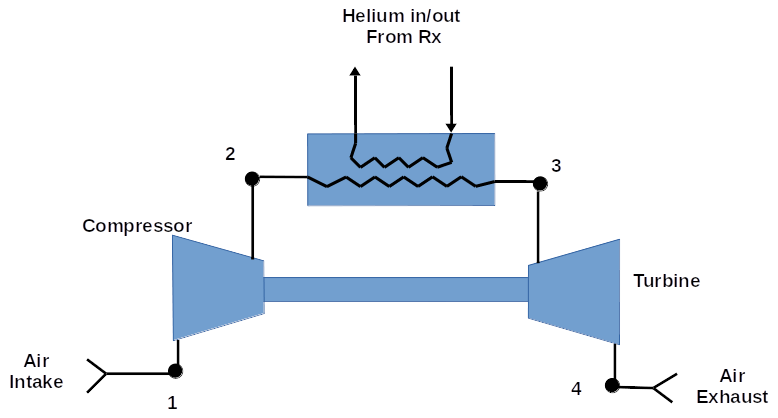
\includegraphics{simple_brayton_ex_schematic.png}
\caption{Open, indirect Brayton cycle.}
\label{fig:simple_brayton_ex_schematic}
\end{marginfigure}



\begin{example}
\textbf{Example:} A small modular reactor concept is proposed in which a helium-cooled, graphite moderated reactor transfers energy in a heat exchanger to an open Brayton cycle as depicted below.  A schematic is shown in Figure \ref{fig:simple_brayton_ex_schematic}. Air at 14.7 psia and 60$^{\circ}$F enters the compressor, passes through the heat exchanger at constant pressure and expands through a turbine that exhausts to the atmosphere.  The compressor has a pressure ratio of 14 and the turbine inlet temperature is 1600$^{\circ}$F. Compressor isentropic efficiency is 87\% and the turbine isentropic efficiency is 90\%.  

Find:

\begin{enumerate}
\item net specific work
\item cycle thermal efficiency; and
\item back work ratio
\end{enumerate}
\end{example} 

\newthought{This example considers} an indirect, open Brayton cycle that uses air for the working fluid.  The solution will be found using EasyProp with, in this case, the entirety of the analysis code included.  A state point table summarizing the thermodynamic properties after each process in the cycle  and numeric results are provided in Figure \ref{fig:simple_brayton_ex_sol}.

\begin{marginfigure}
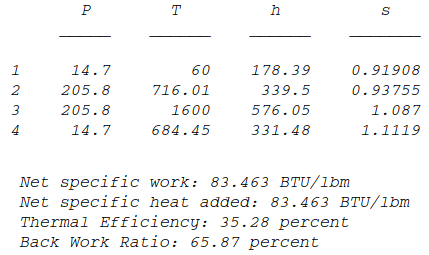
\includegraphics{simple_brayton_ex_results.png}
\caption{Numeric results}
\label{fig:simple_brayton_ex_sol}
\end{marginfigure}

\textbf{Solution:}
Full solution code is provided in the listing below.
\begin{lstlisting}
%% Open, Indirect, Air Brayton Cycle Example
clear
clc
close 'all'

%% Put EasyProp on Python path
% put location of EasyProp.py module on the python search path
if count(py.sys.path,' ') == 0  % <-- see if desired directory is on path
    insert(py.sys.path,int32(0),' '); %<-- if not; add it.
end

%% Initialize Fluid Property object
fluid = 'Air';
units = 'USCS';
air = py.EasyProp.simpleFluid(fluid,units);

%% Initialize state point arrays for Brayton Cycle
numSP = 4;
h = nan(numSP,1);
hs = nan(numSP,1);
s = nan(numSP,1);
ss = nan(numSP,1);
T = nan(numSP,1);
P = nan(numSP,1);

%% Problem Parameters
Pmin = 14.7; % psia, atmospheric pressure
Tin = 60; % F, inlet air temperature
r_p = 14;
r_e = 1/r_p;
T_turb_inlet = 1600; % F

eta_c = 0.87;
eta_t = 0.9;

%% Compute State Point Property Data
% state point 1
P(1) = Pmin;
T(1) = Tin;
h(1) = air.h_pT(P(1),T(1));
s(1) = air.s_pT(P(1),T(1));

% state point 2
P(2) = P(1)*r_p;
ss(2) = s(1);
hs(2) = air.h_ps(P(2),ss(2));
h(2) = h(1) - (h(1)-hs(2))./eta_c;
T(2) = air.T_ph(P(2),h(2));
s(2) = air.s_ph(P(2),h(2));

% state point 3
P(3) = P(2); %isobaric heat addition
T(3) = T_turb_inlet; % F, given
h(3) = air.h_pT(P(3),T(3));
s(3) = air.s_pT(P(3),T(3));

% state point 4
P(4) = P(3)*r_e;
ss(4) = s(3); 
hs(4) = air.h_ps(P(4),ss(4));
h(4) = h(3)-(h(3)-hs(4))*eta_t;
T(4) = air.T_ph(P(4),h(4));
s(4) = air.s_ph(P(4),h(4));

% display state point data neatly
SP = {'1','2','3','4'};
SP_table = table(P,T,h,s,'RowName',SP);
disp(SP_table);

%% First Law Analysis
w_c = h(1) - h(2);
w_t = h(3) - h(4);
w_net = w_c + w_t;

q_s = h(3) - h(2);
q_r = h(1) - h(4);
q_net = q_s + q_r;

assert(abs(w_net - q_net)<1,'Conservation of energy condition not met!');

fprintf('Net specific work: %g BTU/lbm \n',w_net);
fprintf('Net specific heat added: %g BTU/lbm \n',q_net);


eta_th = w_net/q_s;

fprintf('Thermal Efficiency: %5.2f percent \n',eta_th*100);

BWR = abs(w_c/w_t);
fprintf('Back Work Ratio: %5.2f percent \n',BWR*100);
\end{lstlisting}




